\chapter{Modelado clásico: SARIMA}
\label{cap:sarima}

En este capítulo se desarrolla el segundo objetivo específico: la construcción de un modelo estadístico clásico y la evaluación de su capacidad de pronóstico. Este modelo sirve como referencia para los modelos de aprendizaje automático del capítulo~\ref{cap:ml}.

\section{Justificación del modelo}

El análisis exploratorio mostró que el nivel del precio tiene raíz unitaria en buena parte de las series, que muchas de ellas presentan un ciclo anual y que el cambio de un mes está correlacionado con el de los meses anteriores. El modelo SARIMA \eqref{eq:sarima} incorpora estos tres elementos mediante diferencias regulares y estacionales y términos autorregresivos y de medias móviles, y es el modelo de referencia habitual para series mensuales \citep{box2015}.

\section{Especificación y estimación}

Dado el número de series (1\,260), los órdenes se seleccionaron de forma automática con el procedimiento de \citet{hyndman2008auto}, implementado en la librería statsforecast \citep{garza2022}, que elige para cada serie la especificación con menor criterio de información de Akaike corregido, AICc \citep{hurvich1989}. El número de diferencias regulares se decide con la prueba KPSS y el de diferencias estacionales, con una prueba de estacionalidad. El modelo se estimó sobre el logaritmo del precio con los datos disponibles hasta cada corte, y los huecos se completaron únicamente con información anterior al corte. Durante el pronóstico los parámetros se mantuvieron fijos y el modelo se actualizó con cada nuevo precio observado, al igual que los demás modelos. La probabilidad de alza se calculó sumando al pronóstico los errores históricos de la serie y contando la proporción de casos que superan el 15\pct. Los modelos se estimaron en los tres cortes de validación y en el corte de prueba.

\section{Ejemplo: el mango Tommy en Medellín}

Para el mango Tommy de la Central Mayorista de Antioquia el procedimiento seleccionó un modelo SARIMA$(0,0,1)(0,1,1)_{12}$, con una diferencia estacional y un término de medias móviles regular y otro estacional. Se trata de una especificación habitual en series con un ciclo anual marcado.

Como se observa en la figura~\ref{fig:sarima_ejemplo}, el modelo reproduce el ciclo anual del precio, aunque con cierto retraso en algunos cambios de dirección, y la mayoría de los precios observados se ubica dentro del intervalo del 80\pct. En el periodo de prueba, su error absoluto medio fue de 22,3 puntos, frente a 35,2 del último precio y 19,6 de CatBoost.

\begin{figure}[htbp]\centering
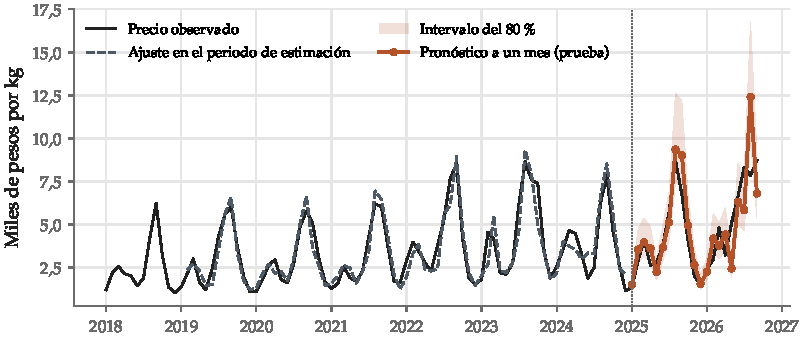
\includegraphics[width=.8\textwidth]{fig_sarima_ejemplo}
\caption{SARIMA$(0,0,1)(0,1,1)_{12}$ para el precio del mango Tommy en la Central Mayorista de Antioquia: ajuste en el periodo de estimación (hasta diciembre de 2024) y pronósticos a un mes en la prueba con un intervalo del 80\pct\ construido con los errores del ajuste.}\label{fig:sarima_ejemplo}
\end{figure}

Los residuos del ajuste oscilan alrededor de cero, sin valores atípicos marcados, sus autocorrelaciones se encuentran dentro de la banda de no significancia al 95\pct\ y la prueba de Ljung--Box \citep{ljung1978} no rechaza la hipótesis de ruido blanco ($p=0{,}39$ con 12 rezagos).


\section{Resultados en el conjunto de series}

La tabla~\ref{tab:sarima} resume las especificaciones seleccionadas con datos hasta 2024. Cerca del 88\pct\ de las series incluyó al menos una diferencia regular, bastante más que el \rvadfno\pct\ en que la prueba de Dickey--Fuller no rechazó la raíz unitaria. La diferencia se debe a que el procedimiento automático decide $d$ con la prueba KPSS sobre la serie en nivel con solo una constante, que rechaza la estacionariedad cuando hay tendencia y, por tanto, tiende a diferenciar más. Solo el 42\pct\ incorporó términos estacionales, posiblemente porque con unos seis años de datos el criterio de información penaliza estos parámetros. En una de cada cuatro series se eligió el modelo $(0,1,0)(0,0,0)$, equivalente al pronóstico con el último precio. Los residuos del \rvlbdoce\pct\ de las series no rechazan la hipótesis de ruido blanco con la prueba de Ljung--Box a 12 rezagos, con grados de libertad ajustados por los parámetros estimados ($12-p-q-P-Q$). Si todos los modelos estuvieran bien especificados se esperaría cerca de un 95\pct, de modo que en unos \rvlbesperado\ puntos porcentuales de las series queda autocorrelación sin capturar.

\begin{table}[htbp]\centering\small
\caption{Modelos SARIMA estimados con datos hasta 2024 (corte de la prueba): órdenes elegidos y diagnóstico de residuos}\label{tab:sarima}
\begin{adjustbox}{max width=\textwidth}\begin{tabular}{lr}\toprule
Característica & Valor\\ \midrule
Series estimadas & 1.260 \\
Con una diferencia regular ($d\ge1$) & 87{,}5\,\% \\
Con diferencia estacional ($D\ge1$) & 12{,}8\,\% \\
Con algún término estacional & 42{,}1\,\% \\
Residuos sin autocorrelación (Ljung--Box, 12 rezagos, $p>0{,}05$) & 84{,}5\,\% \\
Residuos sin autocorrelación (Ljung--Box, 24 rezagos, $p>0{,}05$) & 83{,}7\,\% \\
\midrule
\multicolumn{2}{l}{Órdenes más frecuentes $(p,d,q)(P,D,Q)_{12}$} \\
\quad (0,1,0)(0,0,0) & 24{,}7\,\% \\
\quad (1,1,0)(0,0,0) & 5{,}2\,\% \\
\quad (0,1,1)(0,0,0) & 5{,}0\,\% \\
\quad (2,1,1)(0,0,0) & 3{,}5\,\% \\
\quad (0,1,2)(0,0,0) & 3{,}3\,\% \\
\quad (1,1,1)(0,0,0) & 3{,}1\,\% \\
\bottomrule\end{tabular}\end{adjustbox}\end{table}


En la validación (2022--2024), el error del SARIMA fue mayor que el del último precio en el agregado (tabla~\ref{tab:sarima_error}). El resultado depende del año: en 2022 el SARIMA tuvo un error un \rvsaraabs\pct\ mayor que el último precio, mientras que en 2023 y 2024 lo redujo en un \rvsarb\pct\ y un \rvsarc\pct. En el periodo de prueba redujo el error del último precio en un \cmejsar\pct. La tabla usa la misma definición que la tabla principal de resultados (promedio de los tres años y, donde el SARIMA no pudo estimarse, el último precio; en 2022 se estimó en el \rvsardisp\pct\ de los casos), por lo que sus cifras coinciden con las de la tabla~\ref{tab:reg}. Esta variación entre años indica que la ganancia del modelo depende de la similitud entre el ciclo de los años recientes y el de los años de estimación.

\begin{table}[htbp]\centering\small
\caption{MAE (puntos porcentuales) del último precio y del SARIMA y reducción del error del SARIMA (\%). Validación: promedio de los MAE de 2022, 2023 y 2024, con la misma definición que la tabla~\ref{tab:reg} (donde el SARIMA no pudo estimarse se usa el último precio).}\label{tab:sarima_error}
\begin{adjustbox}{max width=\textwidth}\begin{tabular}{lrrrrrr}\toprule
& \multicolumn{3}{c}{Validación} & \multicolumn{3}{c}{Prueba}\\ \cmidrule(lr){2-4}\cmidrule(lr){5-7}
Grupo & Últ. precio & SARIMA & Reducción & Últ. precio & SARIMA & Reducción\\ \midrule
Todo el panel & 13{,}31 & 13{,}51 & \ensuremath{-}1{,}5 & 12{,}06 & 11{,}50 & 4{,}7 \\ \midrule
Verduras y hortalizas & 17{,}18 & 18{,}04 & \ensuremath{-}5{,}0 & 16{,}33 & 15{,}87 & 2{,}8 \\
Tubérculos y plátanos & 12{,}81 & 14{,}02 & \ensuremath{-}9{,}4 & 12{,}35 & 12{,}16 & 1{,}5 \\
Frutas & 13{,}79 & 12{,}99 & 5{,}8 & 11{,}91 & 10{,}89 & 8{,}6 \\
Lácteos y huevos & 4{,}57 & 4{,}81 & \ensuremath{-}5{,}3 & 3{,}54 & 3{,}54 & 0{,}1 \\
Pescados & 4{,}05 & 5{,}28 & \ensuremath{-}30{,}3 & 3{,}36 & 3{,}95 & \ensuremath{-}17{,}4 \\
Granos y cereales & 3{,}36 & 4{,}22 & \ensuremath{-}25{,}8 & 2{,}75 & 2{,}86 & \ensuremath{-}3{,}8 \\
Procesados & 2{,}54 & 2{,}72 & \ensuremath{-}7{,}0 & 2{,}00 & 2{,}07 & \ensuremath{-}3{,}5 \\
\midrule \multicolumn{7}{l}{\emph{Validación por año (todo el panel)}}\\
\quad 2022 & 13{,}41 & 15{,}93 & \ensuremath{-}18{,}8 & & & \\
\quad 2023 & 12{,}89 & 12{,}01 & 6{,}8 & & & \\
\quad 2024 & 13{,}62 & 12{,}59 & 7{,}6 & & & \\
\bottomrule\end{tabular}\end{adjustbox}\end{table}


\section{Conclusiones del modelado clásico}

El SARIMA presenta un buen ajuste a nivel de serie y reproduce el ciclo anual cuando este es marcado. No obstante, su mejora frente al último precio es pequeña y varía entre periodos. Dos limitaciones explican este resultado: cada modelo utiliza únicamente la historia de su propia serie y, con pocos años de datos, los componentes estacionales se estiman con baja precisión. Estos resultados motivan el uso de modelos que aprovechen la información conjunta de todas las series.

\FloatBarrier
